\section{Description of the reference frames}
In order to synthesize the controllers laws four reference frames must be define.
\begin{figure}[h]
  \centering
  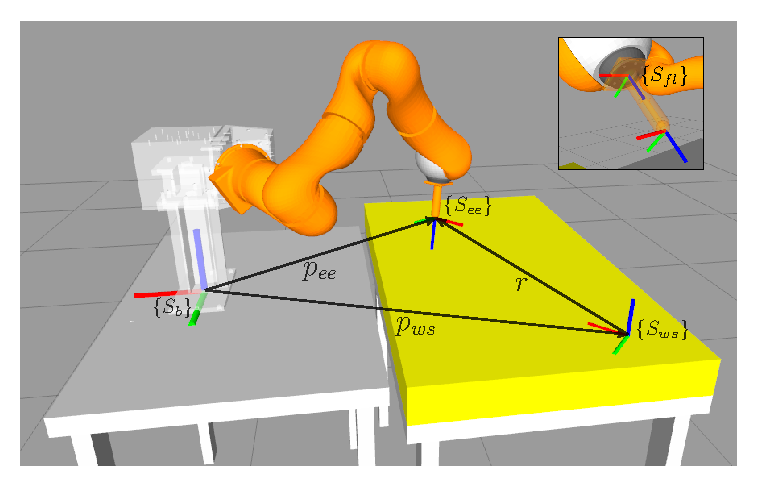
\includegraphics[scale=0.9]{frames.pdf}
  \caption{Reference frames}
\end{figure}
$\{S_{b}\}$ and $\{S_{ws}\}$ are two inertial frames, the first one is placed on the base of the robot's support while the other one is used to easy express reference trajectory.
\[
\begin{split}
  &\{S_b\} = \{B; x_b, y_b, z_b \}\\
  &\{S_{ws}\} = \{W; x_{ws}, y_{ws}, z_{ws} \}\\
\end{split}
\]
Also $\{S_{fl}\}$ and $\{S_{ee}\}$ are defined, the first is placed on the center of the robot wrist and the second on the point of the end-effector with respect the position and the attitude are expressed.
\[
\begin{split}
  &\{S_{fl}\} = \{F; x_{fl}, y_{fl}, z_{fl} \}\\
  &\{S_{ee}\} = \{E; x_{ee}, y_{ee}, z_{ee} \}\\
\end{split}
\]
Furthermore $\vec{p}_{ws}$ is a constant vector used to define the distance between the base frame and the work-space frame, $\vec{p}_{ee}$ is the position vector of the interesting point of the end-effector and the vector $r$ is the distance between the workspace and the end-effector.

Finally the following vector notation will be used $\prescript{y}{}{x}_z$ where $y$ is the reference frames in which the quantity $x$ is expressed and $z$ is the reference point of a wrench or a Jacobian.
%%\begin{frame}
%  \centering
%  \frametitle{Description of the reference frames}
%  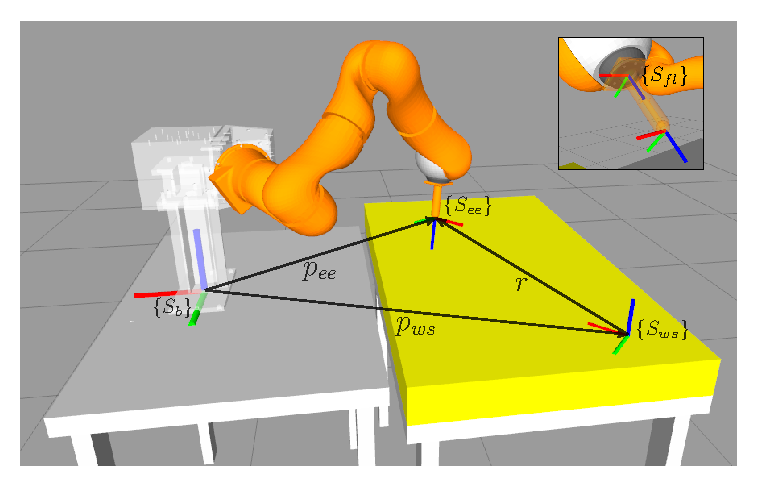
\includegraphics[scale=0.8]{frames}
%  \vskip-1em
%  \begin{columns}
%    \begin{column}{0.1\columnwidth}
%      \begin{flalign*}
%        &\{S_b\} = \{B; x_b, y_b, z_b \}&\\
%        &\{S_{fl}\} = \{F; x_{fl}, y_{fl}, z_{fl} \}&
%      \end{flalign*}
%    \end{column}
%   \begin{column}{0.1\columnwidth}
%     \begin{flalign*}
%        &\{S_{ee}\} = \{E; x_{ee}, y_{ee}, z_{ee} \}&\\
%       &\{S_{ws}\} = \{W; x_{ws}, y_{ws}, z_{ws} \}&
%      \end{flalign*}
%    \end{column}
%  \end{columns}
%\end{frame}
